% Created 2014-06-20 vie 17:19
\documentclass[xcolor={usenames,svgnames,dvipsnames}]{beamer}
\usepackage[utf8]{inputenc}
\usepackage[T1]{fontenc}
\usepackage{fixltx2e}
\usepackage{graphicx}
\usepackage{longtable}
\usepackage{float}
\usepackage{wrapfig}
\usepackage{rotating}
\usepackage[normalem]{ulem}
\usepackage{amsmath}
\usepackage{textcomp}
\usepackage{marvosym}
\usepackage{wasysym}
\usepackage{amssymb}
\usepackage{hyperref}
\tolerance=1000
\usepackage{color}
\usepackage{listings}
\usepackage{gensymb}
\DeclareMathOperator{\sign}{sign}
\lstset{commentstyle=\color{gray!90}, basicstyle=\ttfamily\small, breaklines=true, linewidth=\textwidth, backgroundcolor=\color{gray!10}, basewidth={0.5em,0.4em}, literate={á}{{\'a}}1 {ñ}{{\~n}}1 {é}{{\'e}}1 {ó}{{\'o}}1 {º}{{\textordmasculine}}1}
\usepackage{mathpazo}
\usefonttheme{serif}
\usecolortheme{rose}
\hypersetup{colorlinks=true, linkcolor=Blue!50!black, urlcolor=Blue!50!black, breaklinks=true}
\setbeamercolor{alerted text}{fg=Blue!50!black} \setbeamerfont{alerted text}{series=\bfseries}
\usetheme{default}
\author{Oscar Perpiñán Lamigueiro \\ \url{http://oscarperpinan.github.io}}
\date{GEOSTAT \\ June 2014}
\title{Visualization of raster data with \alert{\texttt{rasterVis}}}
\hypersetup{
  pdfkeywords={},
  pdfsubject={},
  pdfcreator={Emacs 24.3.1 (Org mode 8.2.1)}}
\begin{document}

\maketitle


\begin{frame}[fragile,label=sec-1]{Background}
 \begin{block}{About me}
During the past 15 years, my main area of expertise has been
photovoltaic solar energy systems, with a special interest in solar
radiation.
\end{block}
\begin{block}{I have developed some packages}
\begin{description}
\item[{\href{http://oscarperpinan.github.io/solar}{\texttt{solaR}}}] Solar radiation and performance of photovoltaic systems.
\item[{\href{http://oscarperpinan.github.io/rastervis}{\texttt{rasterVis}}}] Visualization of raster data.
\item[{\href{https://github.com/oscarperpinan/meteoForecast}{\texttt{meteoForecast}}}] (beta) Retrieve NWP-WRF output from Meteogalicia and
OpenMeteo services.
\end{description}
\end{block}
\end{frame}
\begin{frame}[fragile,label=sec-2]{Background}
 \begin{block}{Origins of \alert{\texttt{rasterVis}}}
I started \alert{\texttt{rasterVis}} with Robert Hijmans three years ago when I was
involved in an \href{https://github.com/oscarperpinan/CMSAF-SIAR}{analysis of solar radiation} satellite data (\href{http://wui.cmsaf.eu/safira/action/viewDoiDetails?acronym%3DRAD_MVIRI_V001}{CM SAF}) and ground
measurements (\href{http://eportal.magrama.gob.es/websiar/SeleccionParametrosMap.aspx?dst%3D1}{SIAR})

\begin{description}
\item[{CM SAF}] a \texttt{RasterStack} with 730 layers of daily radiation.
\item[{SIAR}] a set of 300 time series (one for each station) each with
730 records.
\end{description}
\end{block}
\end{frame}

\begin{frame}[label=sec-3]{Background}
\begin{block}{Objectives}
I needed methods to display spatio-temporal raster data and combine it
easily with vector data with \alert{two main objectives}:
\begin{itemize}
\item Understand data
\item Communicate results
\end{itemize}
\end{block}
\end{frame}
\begin{frame}[fragile,label=sec-4]{}
 \begin{block}{The \alert{\texttt{rasterVis}} package complements the \href{http://cran.r-project.org/web/packages/raster}{\texttt{raster}} package, providing a set of methods for enhanced visualization.}
\begin{itemize}
\item \alert{Level and contour plots} of quantitative and categorical data both
for univariate and multivariate rasters.
\item \alert{Exploratory Data Analysis}: Scatterplots, Histograms and Density
plots, Violin and Boxplots, Matrix of scatterplots.
\item \alert{Spatio-temporal rasters}: \href{http://en.wikipedia.org/wiki/Hovm%25C3%25B6ller_diagram}{Hovmöller diagrams}, \href{http://www.perceptualedge.com/blog/?p%3D390}{horizon
graphs}, and time series plots.
\item \alert{Vector fields} using arrows or streamlines.
\end{itemize}
\end{block}
\end{frame}
\begin{frame}[fragile,label=sec-5]{\texttt{rasterVis} is based on \texttt{grid} and \texttt{lattice}}
 \begin{block}{grid}
\begin{itemize}
\item In \texttt{R} there are two systems, traditional and grid graphics.
\item The \texttt{grid} package is a flexible low-level graphics toolbox that
provides more flexibility to modify or add content, better support
for combining different outputs easily, and more possibilities for
interaction.
\end{itemize}
\end{block}
\end{frame}
\begin{frame}[fragile,label=sec-6]{\texttt{rasterVis} is based on \texttt{grid} and \texttt{lattice}}
 \begin{block}{lattice}
\begin{itemize}
\item The \texttt{lattice} package is an implementation of Trellis graphic, a
rectangular array of panels.

\item \texttt{lattice} uses a \emph{formula} interface to define the structure of the
array of panels with the specification of the variables involved in
the plot.

\item The \texttt{latticeExtra} package complements the \texttt{lattice} with the
implementation of layers, and superposition of \texttt{trellis} objects and
layers.
\end{itemize}
\end{block}
\end{frame}

\begin{frame}[fragile,label=sec-7]{\texttt{levelplot}}
 \lstset{language=R,numbers=none}
\begin{lstlisting}
## Solar Radiation (CM SAF)
levelplot(SISmm)
\end{lstlisting}

\begin{center}
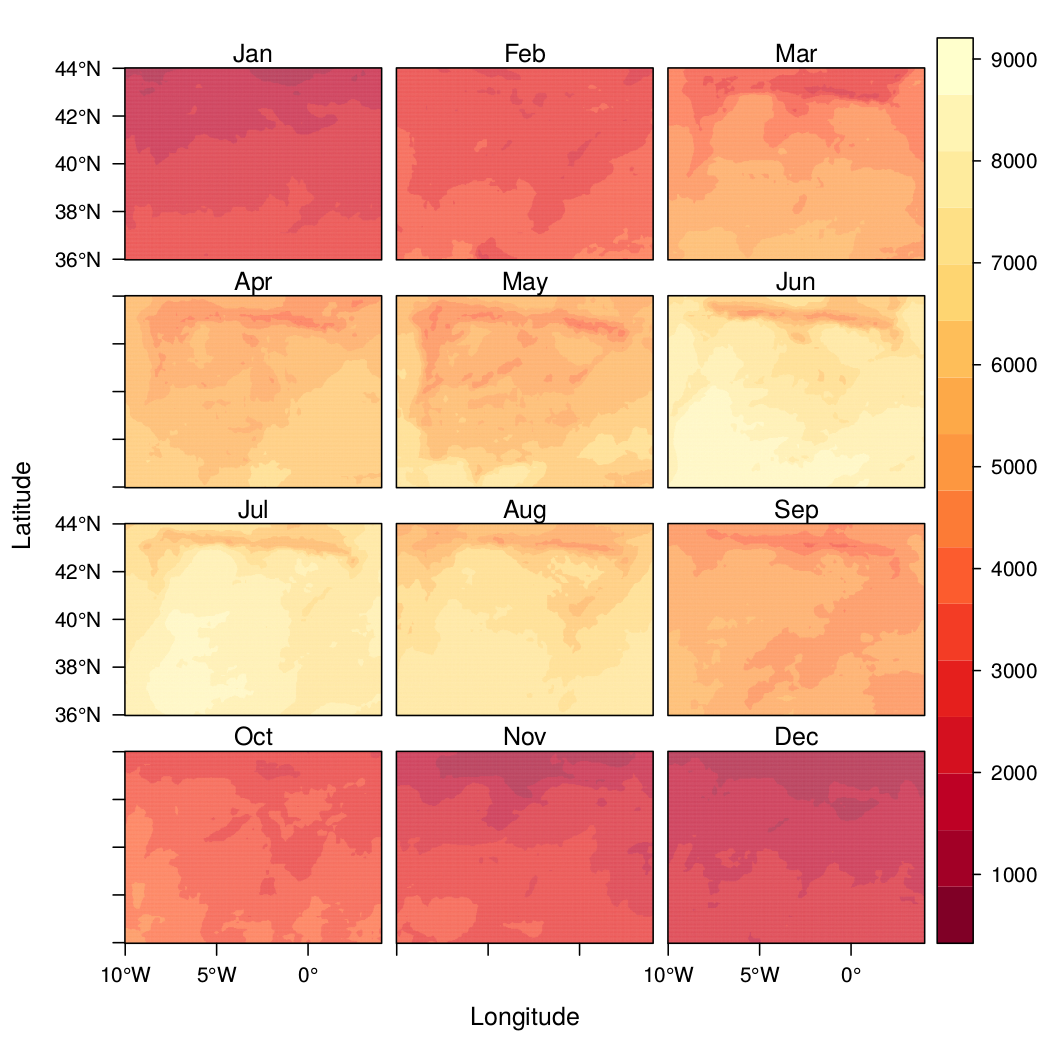
\includegraphics[height=0.65\textheight]{figs/levelplot.png}
\end{center}
\end{frame}
\begin{frame}[fragile,label=sec-8]{Combine raster and vector data}
 \lstset{language=R,numbers=none}
\begin{lstlisting}
levelplot(SISmm, layers = 'Apr') +
    layer(sp.points(spSIAR, pch = 21,
		    fill ='darkgray',
		    col = 'black'))
\end{lstlisting}

\begin{center}
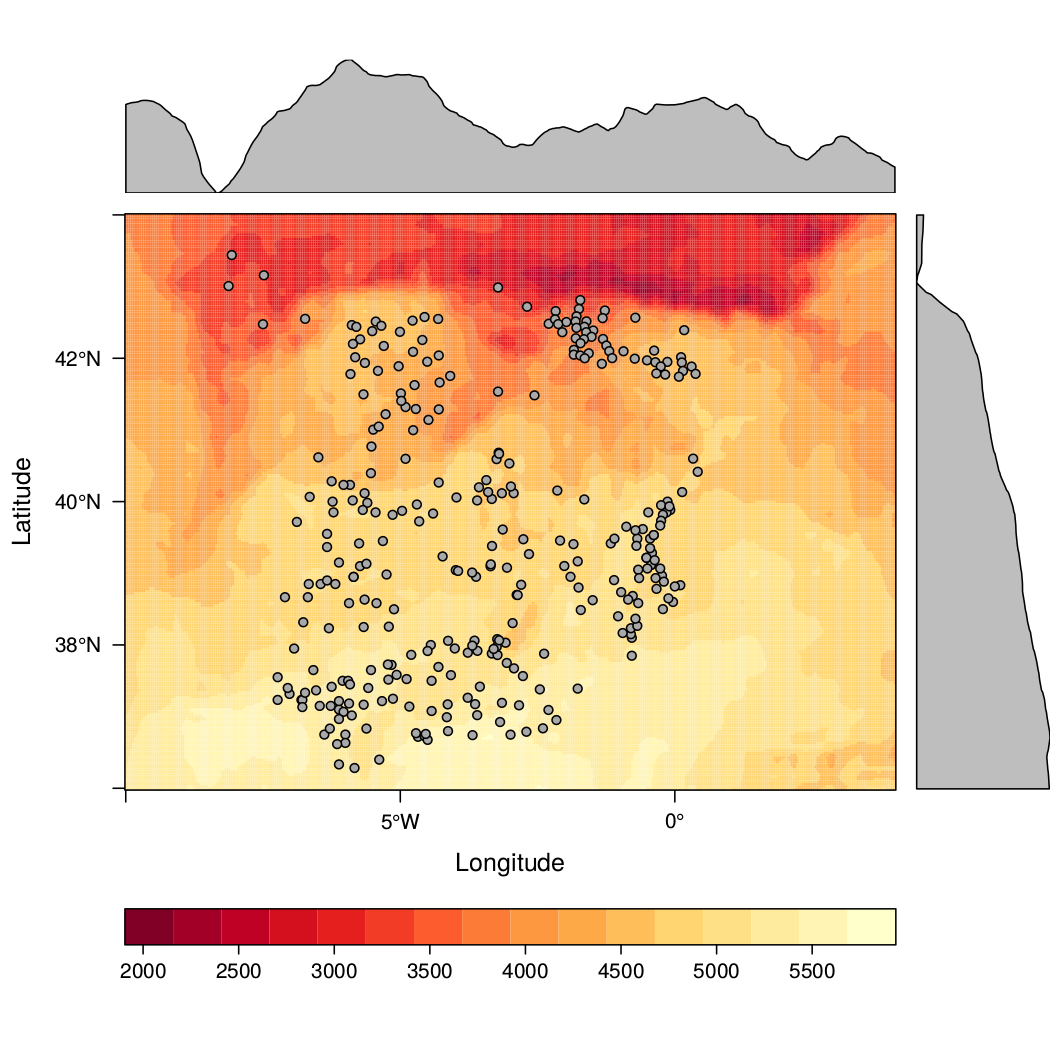
\includegraphics[height=0.65\textheight]{figs/levelplot_points.png}
\end{center}
\end{frame}
\begin{frame}[fragile,label=sec-9]{Movie}
 \lstset{language=R,numbers=none}
\begin{lstlisting}
## Cloud Cover forecasts (MeteoGalicia)

## Create a frame for each layer
trellis.device(png,
	       file=paste0(tmp, '/Rplot%02d.png'))
levelplot(cft, layout=c(1, 1))
dev.off()
## Paste the frames together with ffmpeg
movieCMD <- 'ffmpeg -r 6 -b 300k -i Rplot%02d.png output.mp4'
system(movieCMD)
\end{lstlisting}

\begin{center}
\href{http://player.vimeo.com/video/65227780}{Click here to watch the video}
\end{center}
\end{frame}
\begin{frame}[fragile,label=sec-10]{Themes}
 \lstset{language=R,numbers=none}
\begin{lstlisting}
library(colorspace)
myTheme <- rasterTheme(region=sequential_hcl(10,
			   power=2.2))
levelplot(Aug, par.settings=myTheme,
	  contour=TRUE)
\end{lstlisting}

\begin{center}
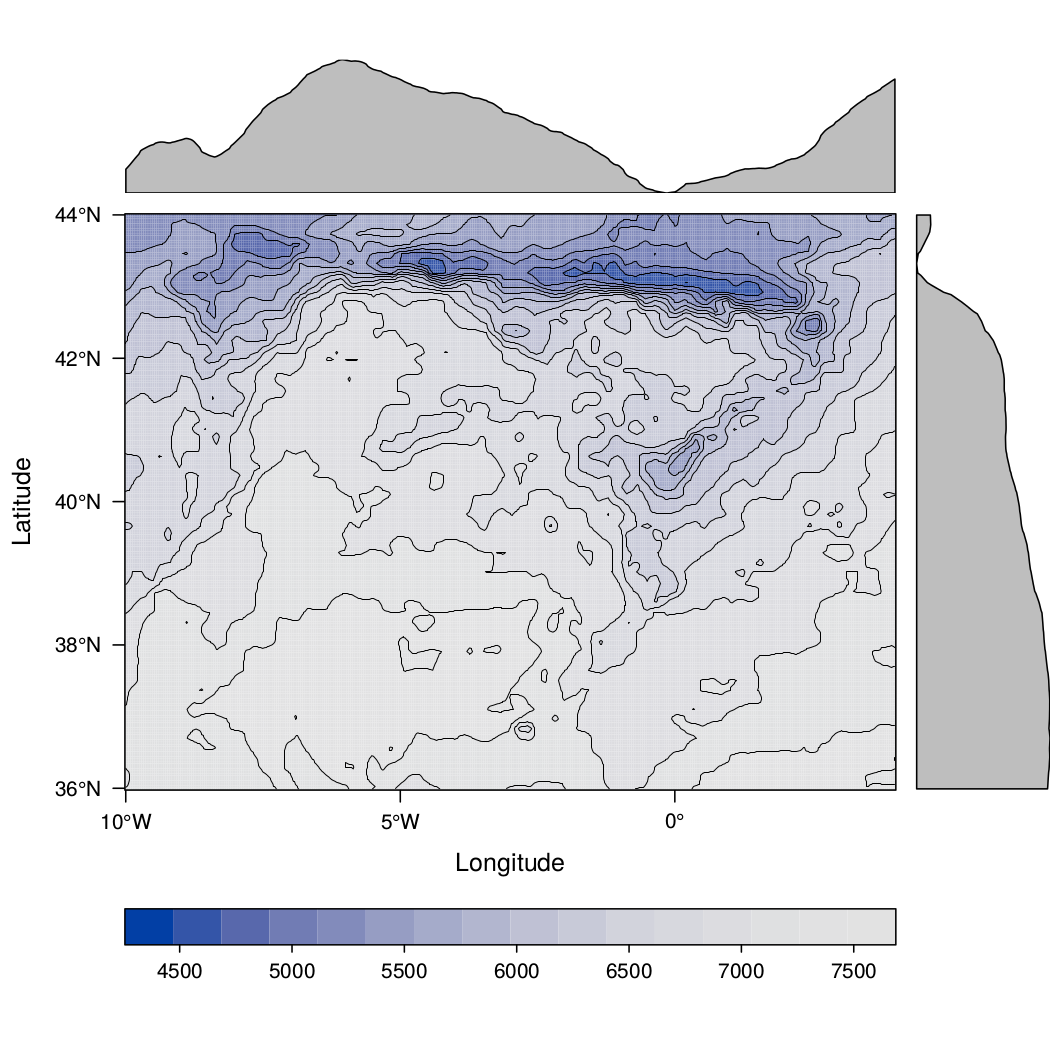
\includegraphics[height=0.65\textheight]{figs/levelplot_colorspace.png}
\end{center}
\end{frame}
\begin{frame}[fragile,label=sec-11]{3D interactive graphics}
 \lstset{language=R,numbers=none}
\begin{lstlisting}
## Digital Elevation Model (Spain)
plot3D(DEM)
\end{lstlisting}

\begin{center}
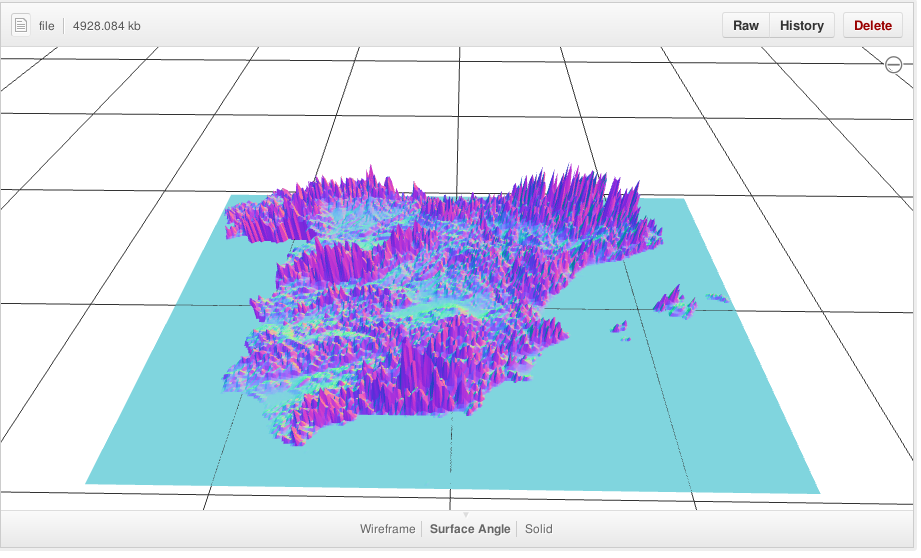
\includegraphics[height=0.5\textheight]{figs/DEM_STL_GitHub.png} 

\href{https://github.com/oscarperpinan/spacetime-vis/blob/gh-pages/images/DEM.stl}{Click here to see the 3D object rendered in GitHub.}
\end{center}
\end{frame}
\begin{frame}[fragile,label=sec-12]{Categorical data}
 \lstset{language=R,numbers=none}
\begin{lstlisting}
## Land cover (NASA)
levelplot(landClass)
\end{lstlisting}

\begin{center}
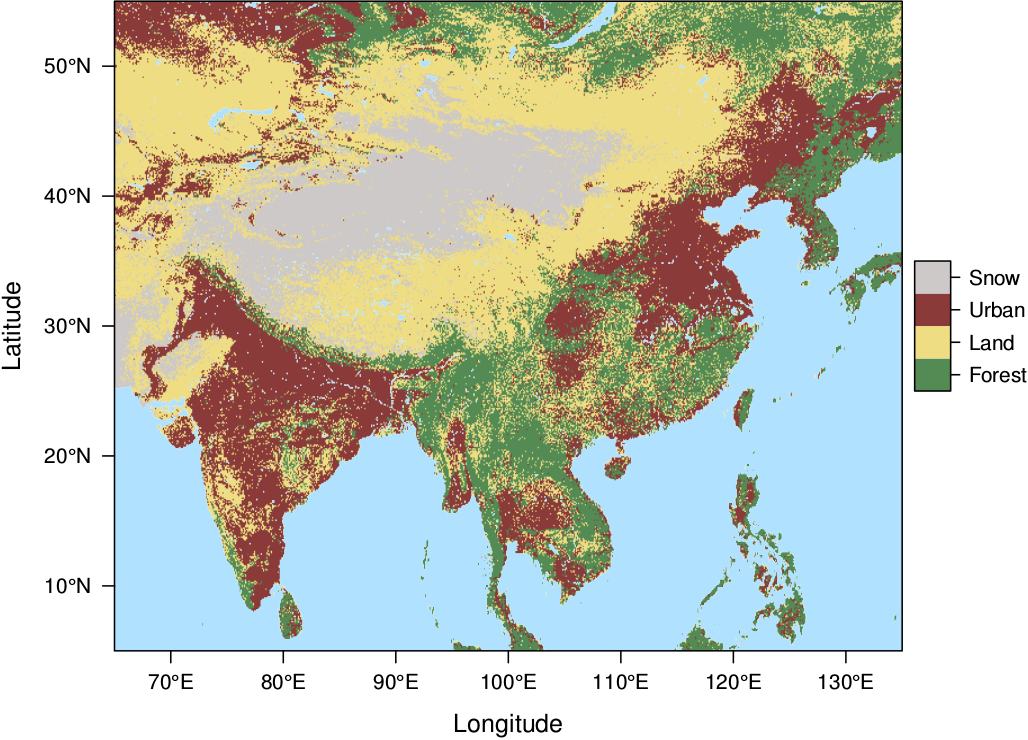
\includegraphics[height=0.65\textheight]{figs/landClass.png}
\end{center}
\end{frame}
\begin{frame}[fragile,label=sec-13]{Scatter plot}
 \lstset{language=R,numbers=none}
\begin{lstlisting}
xyplot(Jan+Feb~Jul|cut(x, 4), data=SISmm,
       auto.key=list(space='right'))
\end{lstlisting}

\begin{center}
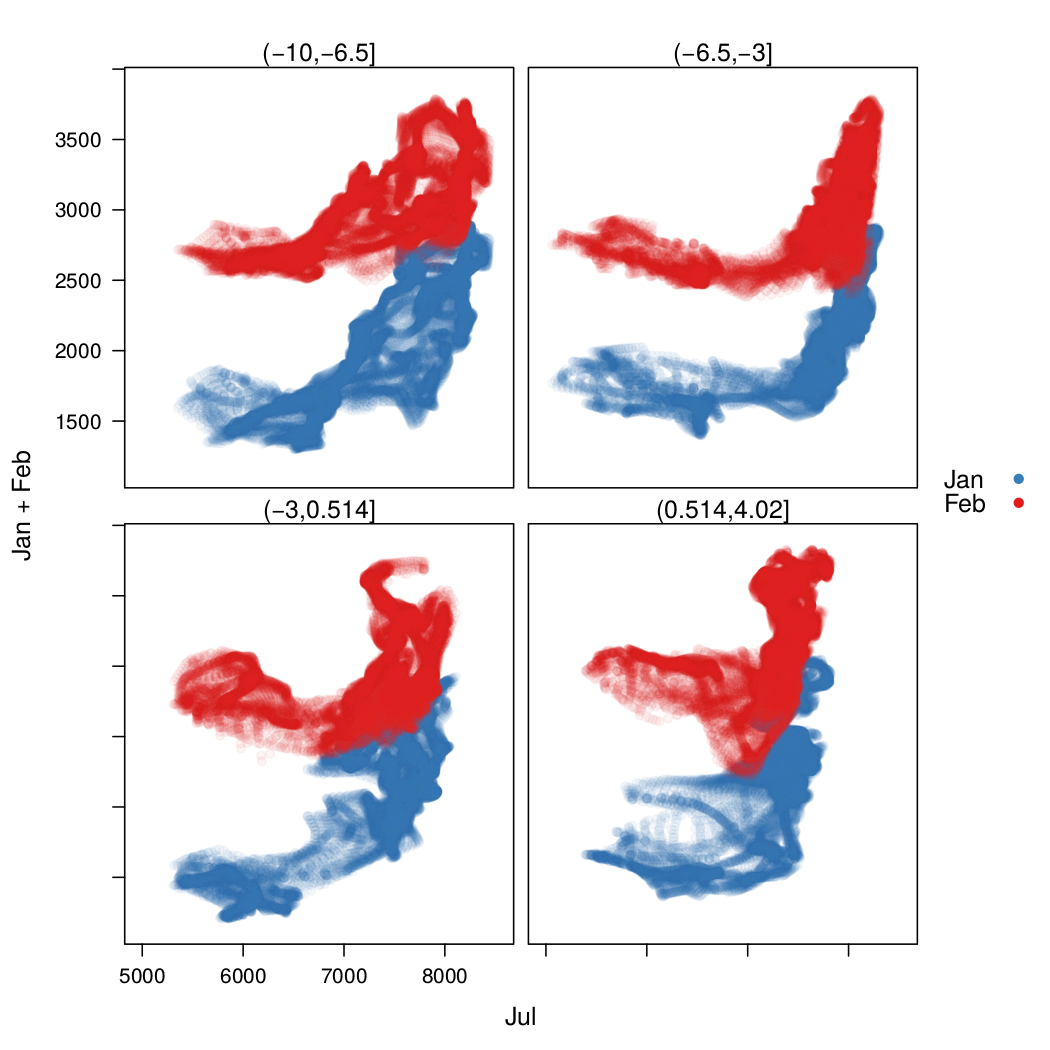
\includegraphics[height=0.65\textheight]{figs/xyplot_formula.png}
\end{center}
\end{frame}
\begin{frame}[fragile,label=sec-14]{Scatter plot matrix}
 \lstset{language=R,numbers=none}
\begin{lstlisting}
splom(SISmm)
\end{lstlisting}

\begin{center}
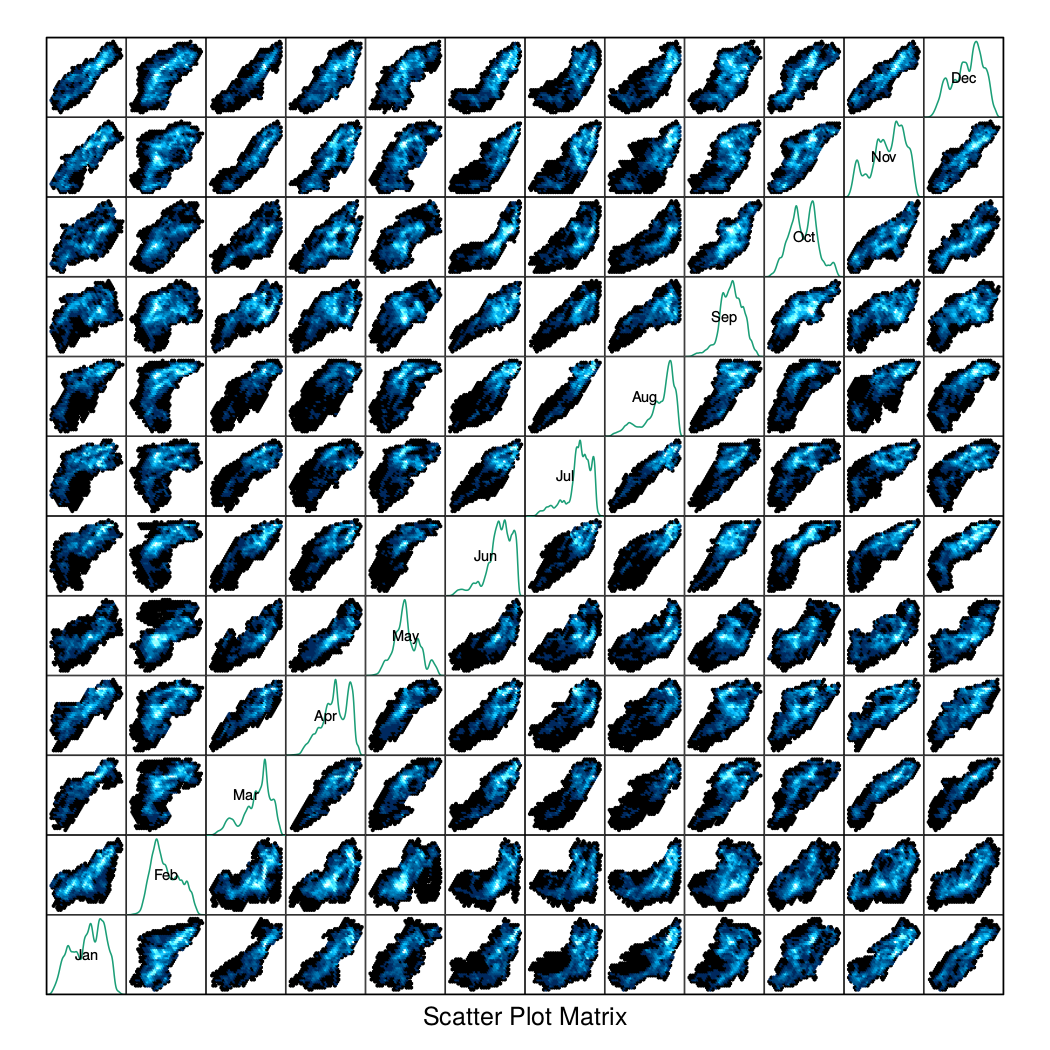
\includegraphics[height=0.65\textheight]{figs/splom.png}
\end{center}
\end{frame}

\begin{frame}[fragile,label=sec-15]{Histograms}
 \lstset{language=R,numbers=none}
\begin{lstlisting}
histogram(SISmm)
\end{lstlisting}

\begin{center}
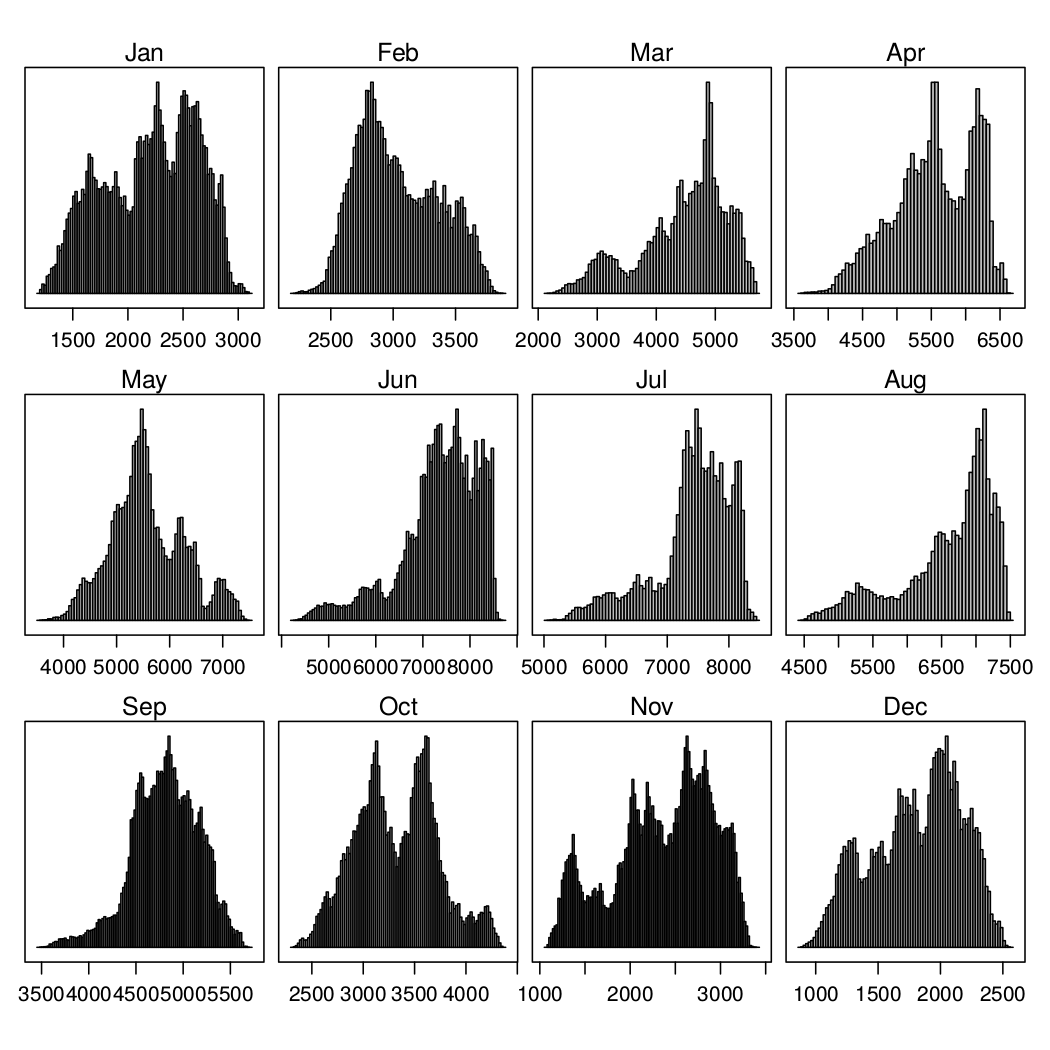
\includegraphics[height=0.65\textheight]{figs/histogram.png}
\end{center}
\end{frame}
\begin{frame}[fragile,label=sec-16]{Hövmoller}
 \lstset{language=R,numbers=none}
\begin{lstlisting}
## Sea Surface Temperature (SST) Anomalies
hovmoller(SST, contour=FALSE,
	  panel = panel.levelplot.raster,
	  yscale.components = yscale.raster.subticks,
	  interpolate = TRUE, par.settings = RdBuTheme)
\end{lstlisting}

\begin{center}
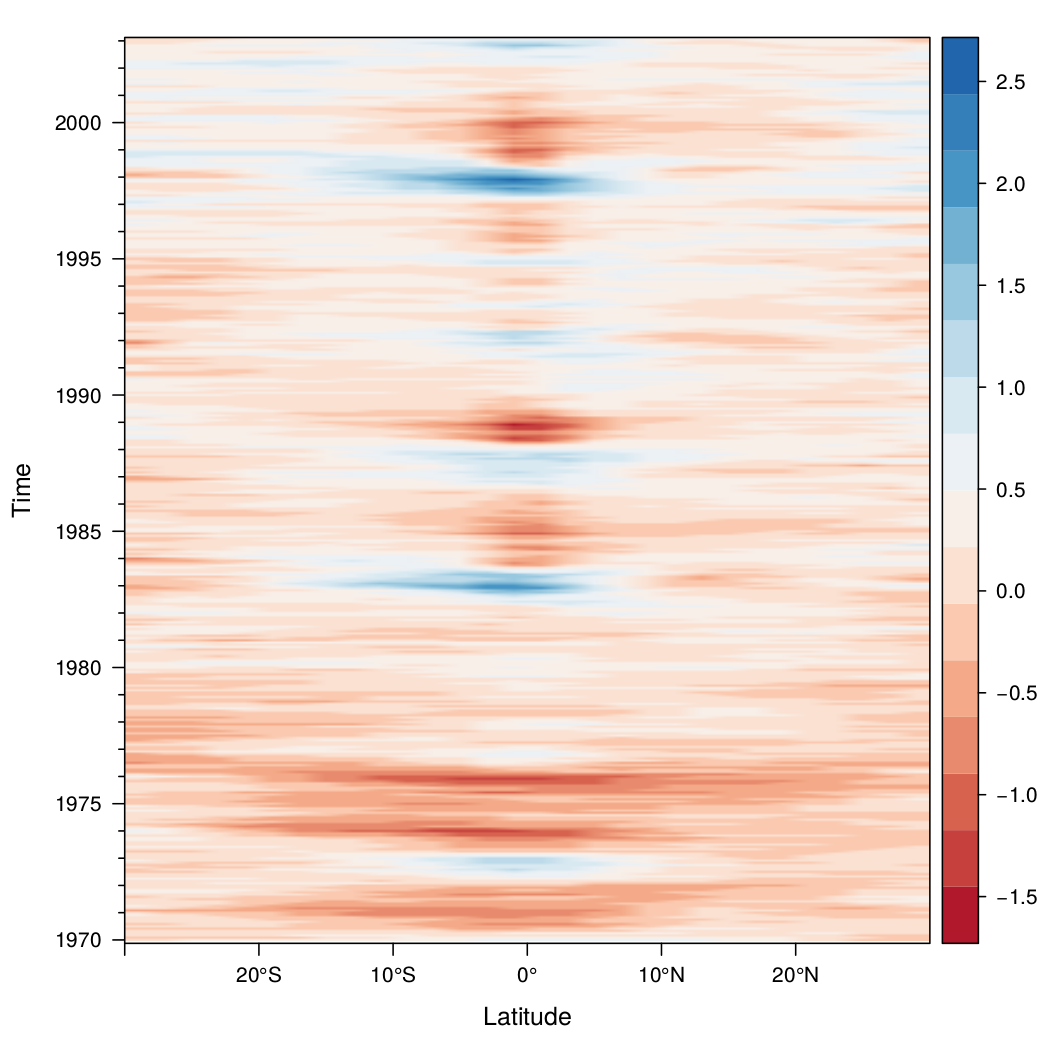
\includegraphics[height=0.65\textheight]{figs/hovmoller.png}
\end{center}
\end{frame}
\begin{frame}[fragile,label=sec-17]{Horizon graph}
 \lstset{language=R,numbers=none}
\begin{lstlisting}
horizonplot(SST)
\end{lstlisting}

\begin{center}
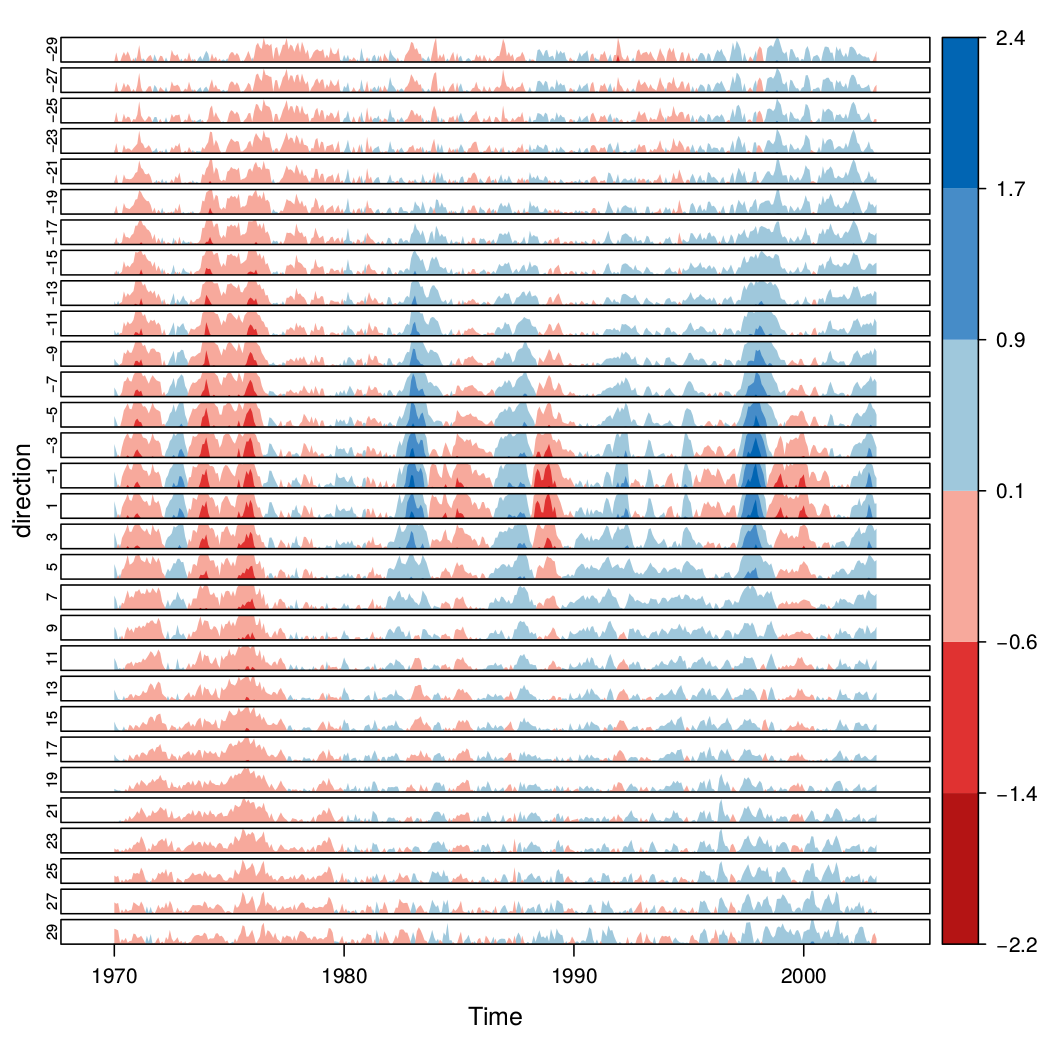
\includegraphics[height=0.65\textheight]{figs/horizon.png}
\end{center}
\end{frame}

\begin{frame}[fragile,label=sec-18]{Vector fields}
 \lstset{language=R,numbers=none}
\begin{lstlisting}
vectorplot(r, par.settings=RdBuTheme())
\end{lstlisting}

\begin{center}
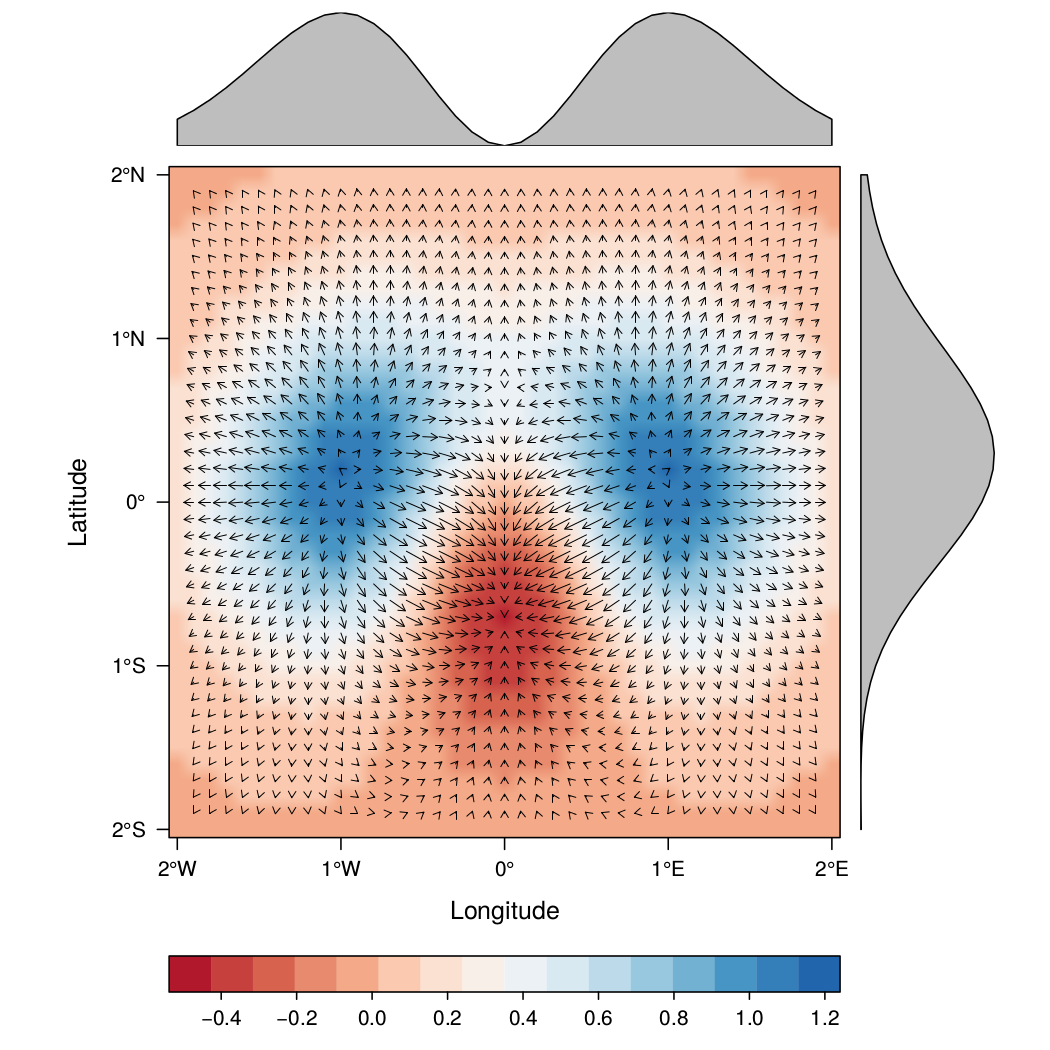
\includegraphics[height=0.65\textheight]{figs/vectorplot.png}
\end{center}
\end{frame}
\begin{frame}[fragile,label=sec-19]{Stream lines}
 \lstset{language=R,numbers=none}
\begin{lstlisting}
streamplot(r2, isField=TRUE,
	   streamlet=list(L=30), droplet=list(pc=.3))
\end{lstlisting}

\begin{center}
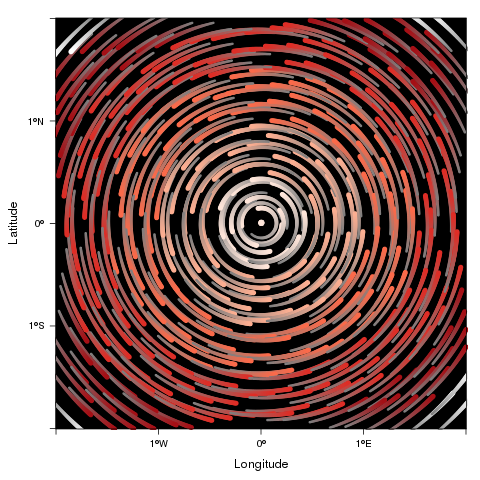
\includegraphics[height=0.65\textheight]{figs/streamplotReds.png}
\end{center}
\end{frame}

\begin{frame}[label=sec-20]{Do you need more?}
\begin{block}{Visit the webpage}
\url{http://oscarperpinan.github.io/rastervis/} (and don't forget the FAQs!)
\end{block}
\begin{block}{I have a book!}
\alert{“Displaying Time Series, Spatial, and Space-Time Data with R”} includes four chapters related to raster data.
Its website offers access to the datasets used in the examples as well as the full R code.
\url{http://oscarperpinan.github.io/spacetime-vis/}

\begin{center}
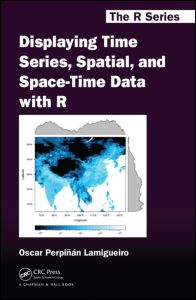
\includegraphics[height=0.3\textwidth]{figs/book.jpg}
\end{center}
\end{block}
\end{frame}
% Emacs 24.3.1 (Org mode 8.2.1)
\end{document}